%----------------------------------------------------------------
%---------------------- Anexos ----------------------------------
%----------------------------------------------------------------

\begin{anexosenv}
\partanexos   % indica o início dos anexos

% Anexo 01
\chapter{Comitê de Ética em Pesquisa}
\begin{center}
    Documento emitido via Plataforma Brasil do Ministério da Saúde.    
\end{center}

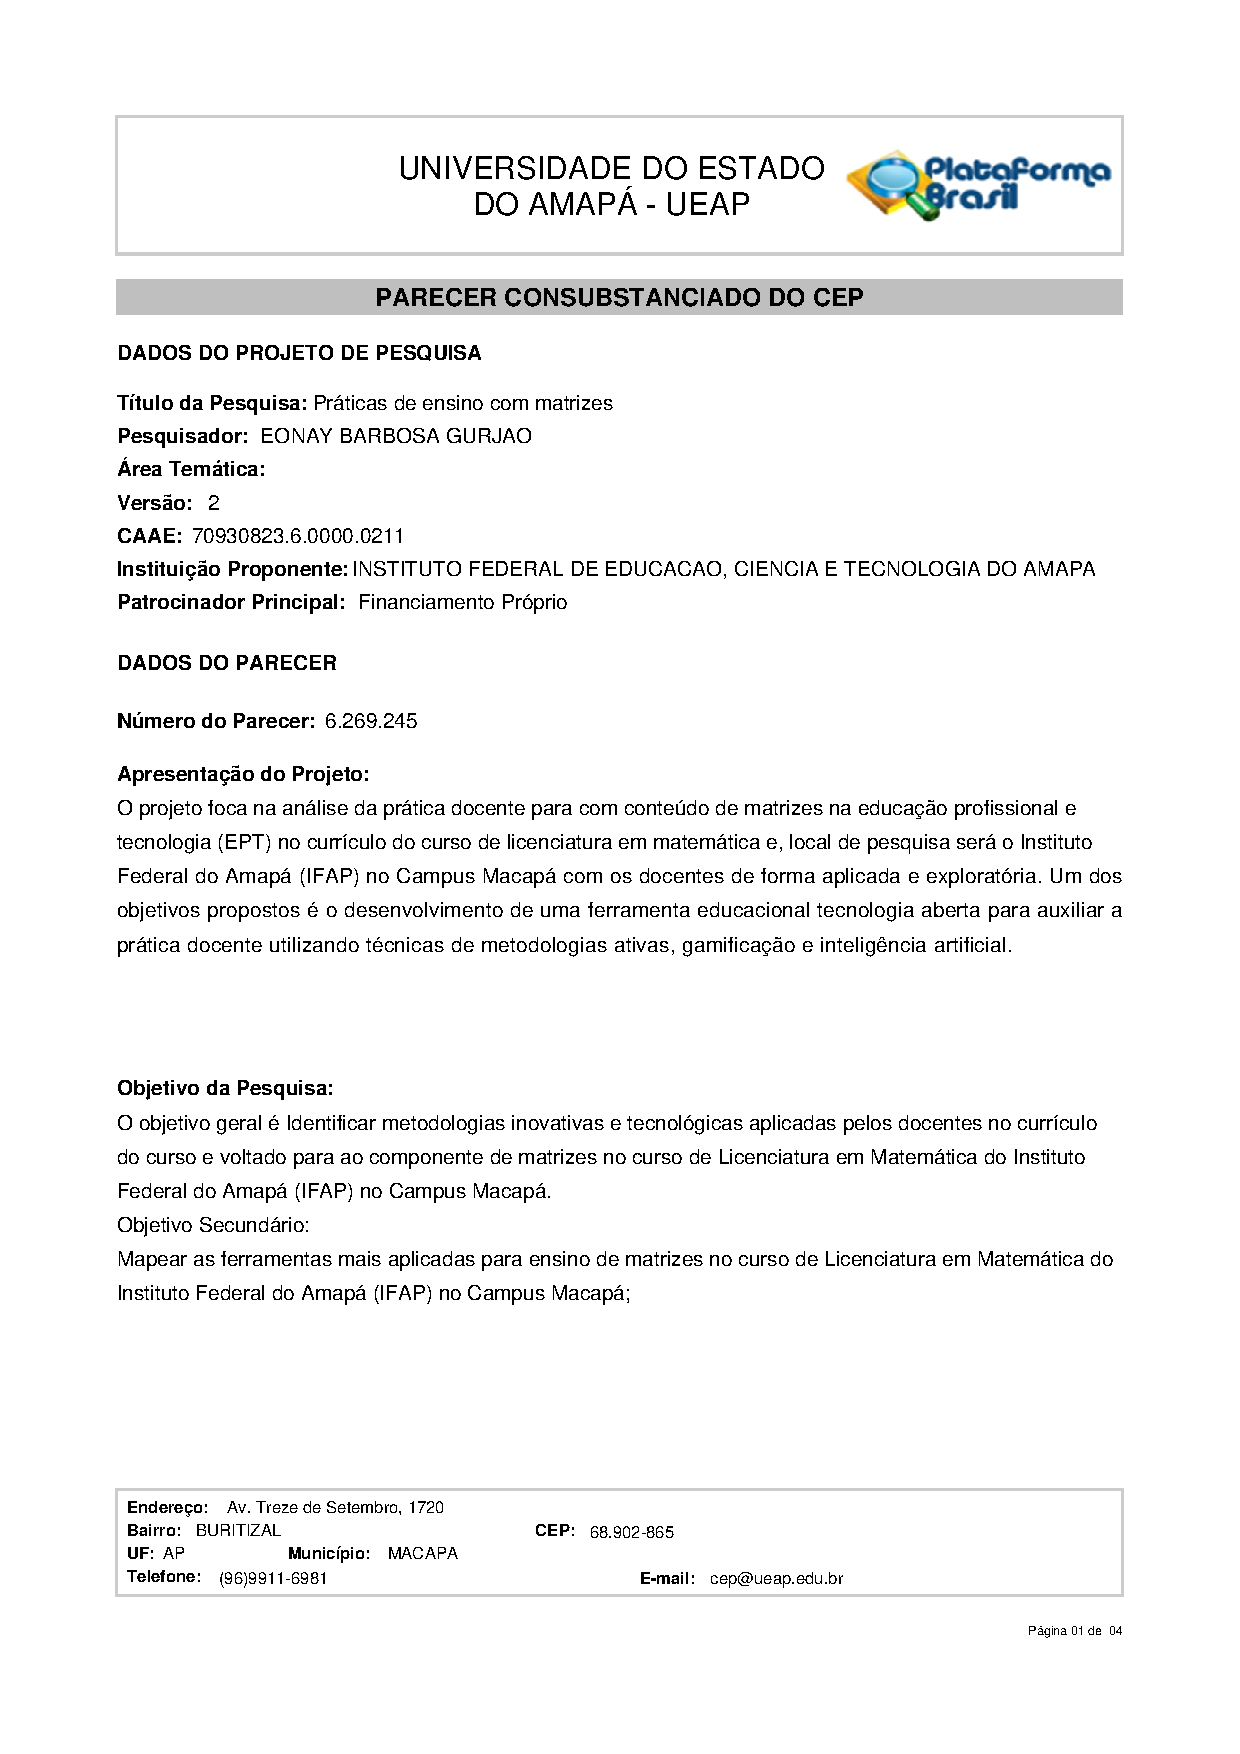
\includepdf[pages=-]{PosTextuais/cep.pdf}


% Anexo 02
\chapter{Termo de Anuência Institucional}
\begin{center}
    Documento emitido via Sistema Unificado de Administração Pública - SUAP do Instituto Federal do Amapá - IFAP.    
\end{center}
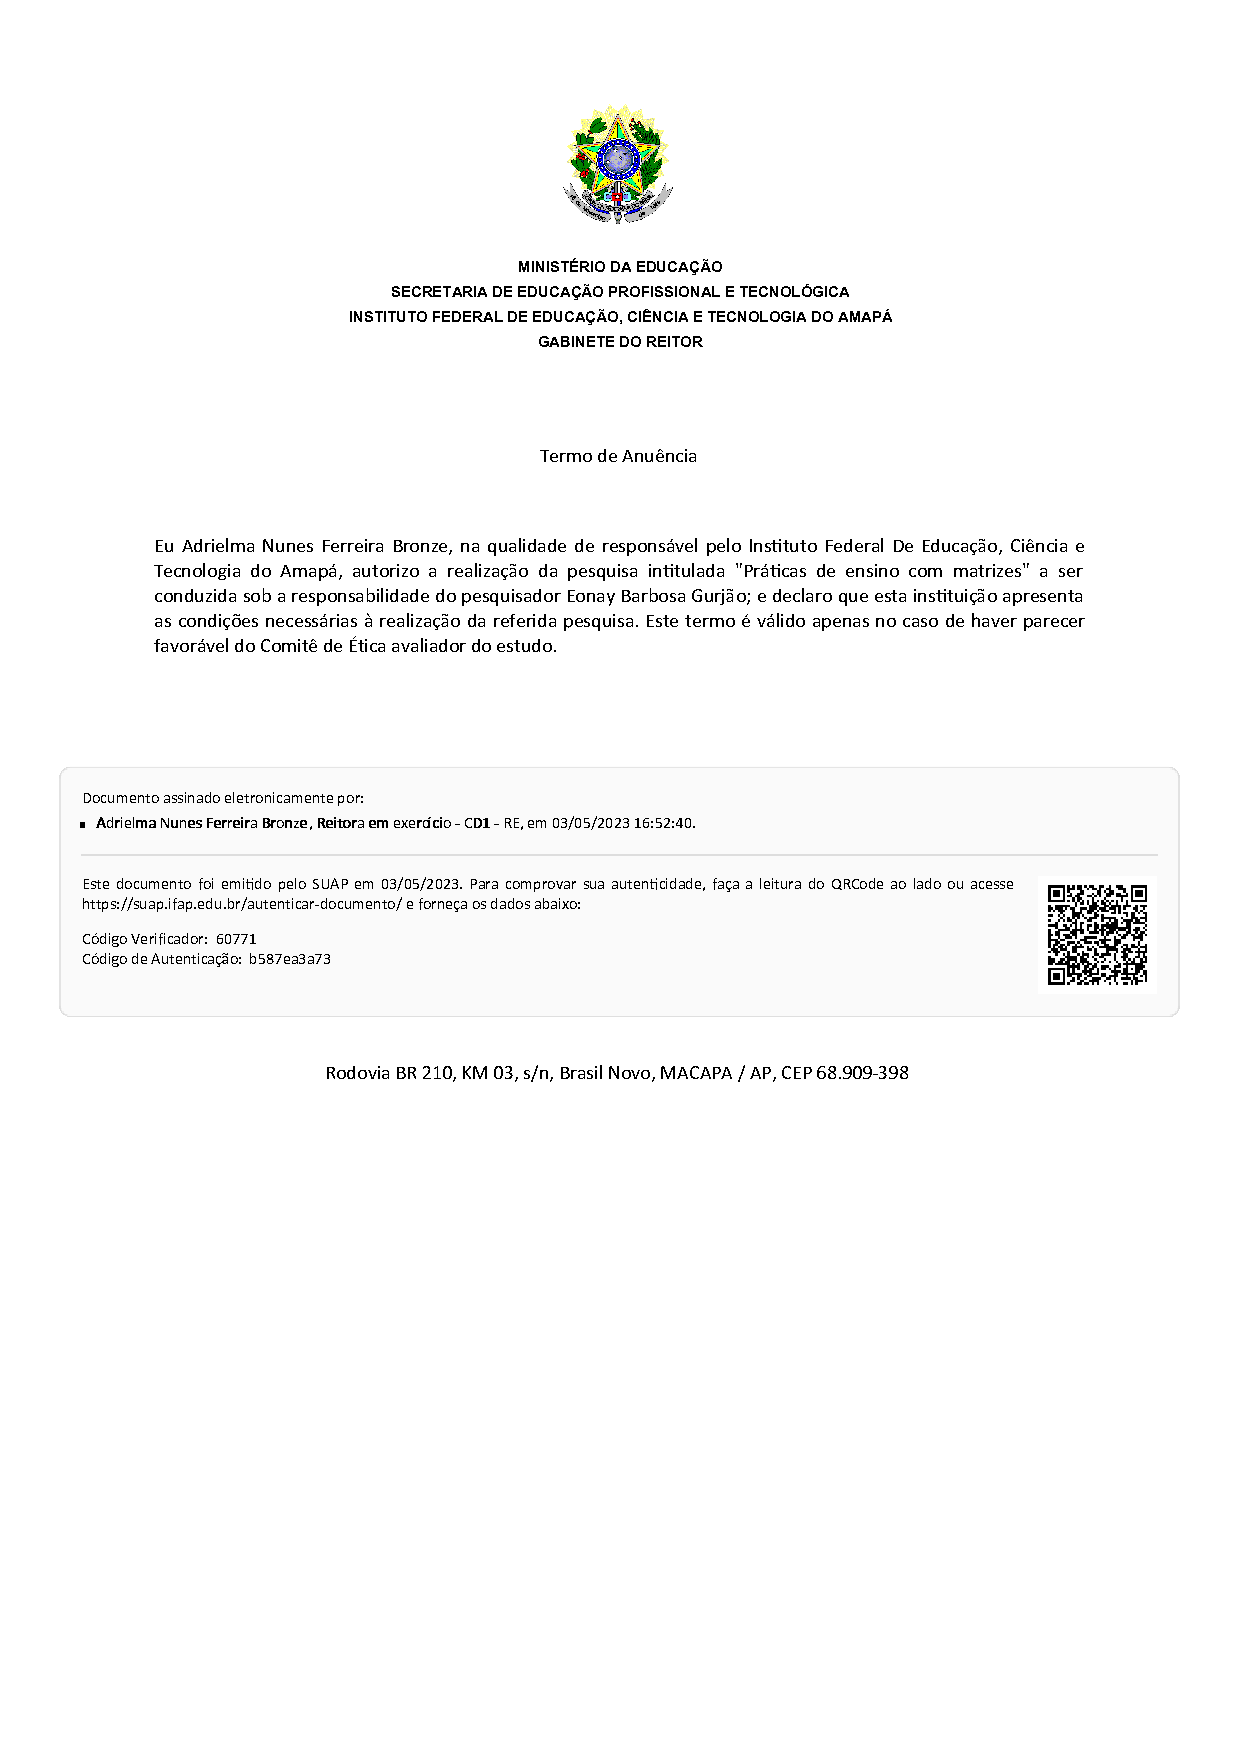
\includepdf[pages=-]{PosTextuais/anuencia.pdf}


% Anexo 03
\chapter{Submissão CNMAC 2023}
\begin{center}
    Documento recebido via Email com o aceite de artigo submetido.    
\end{center}
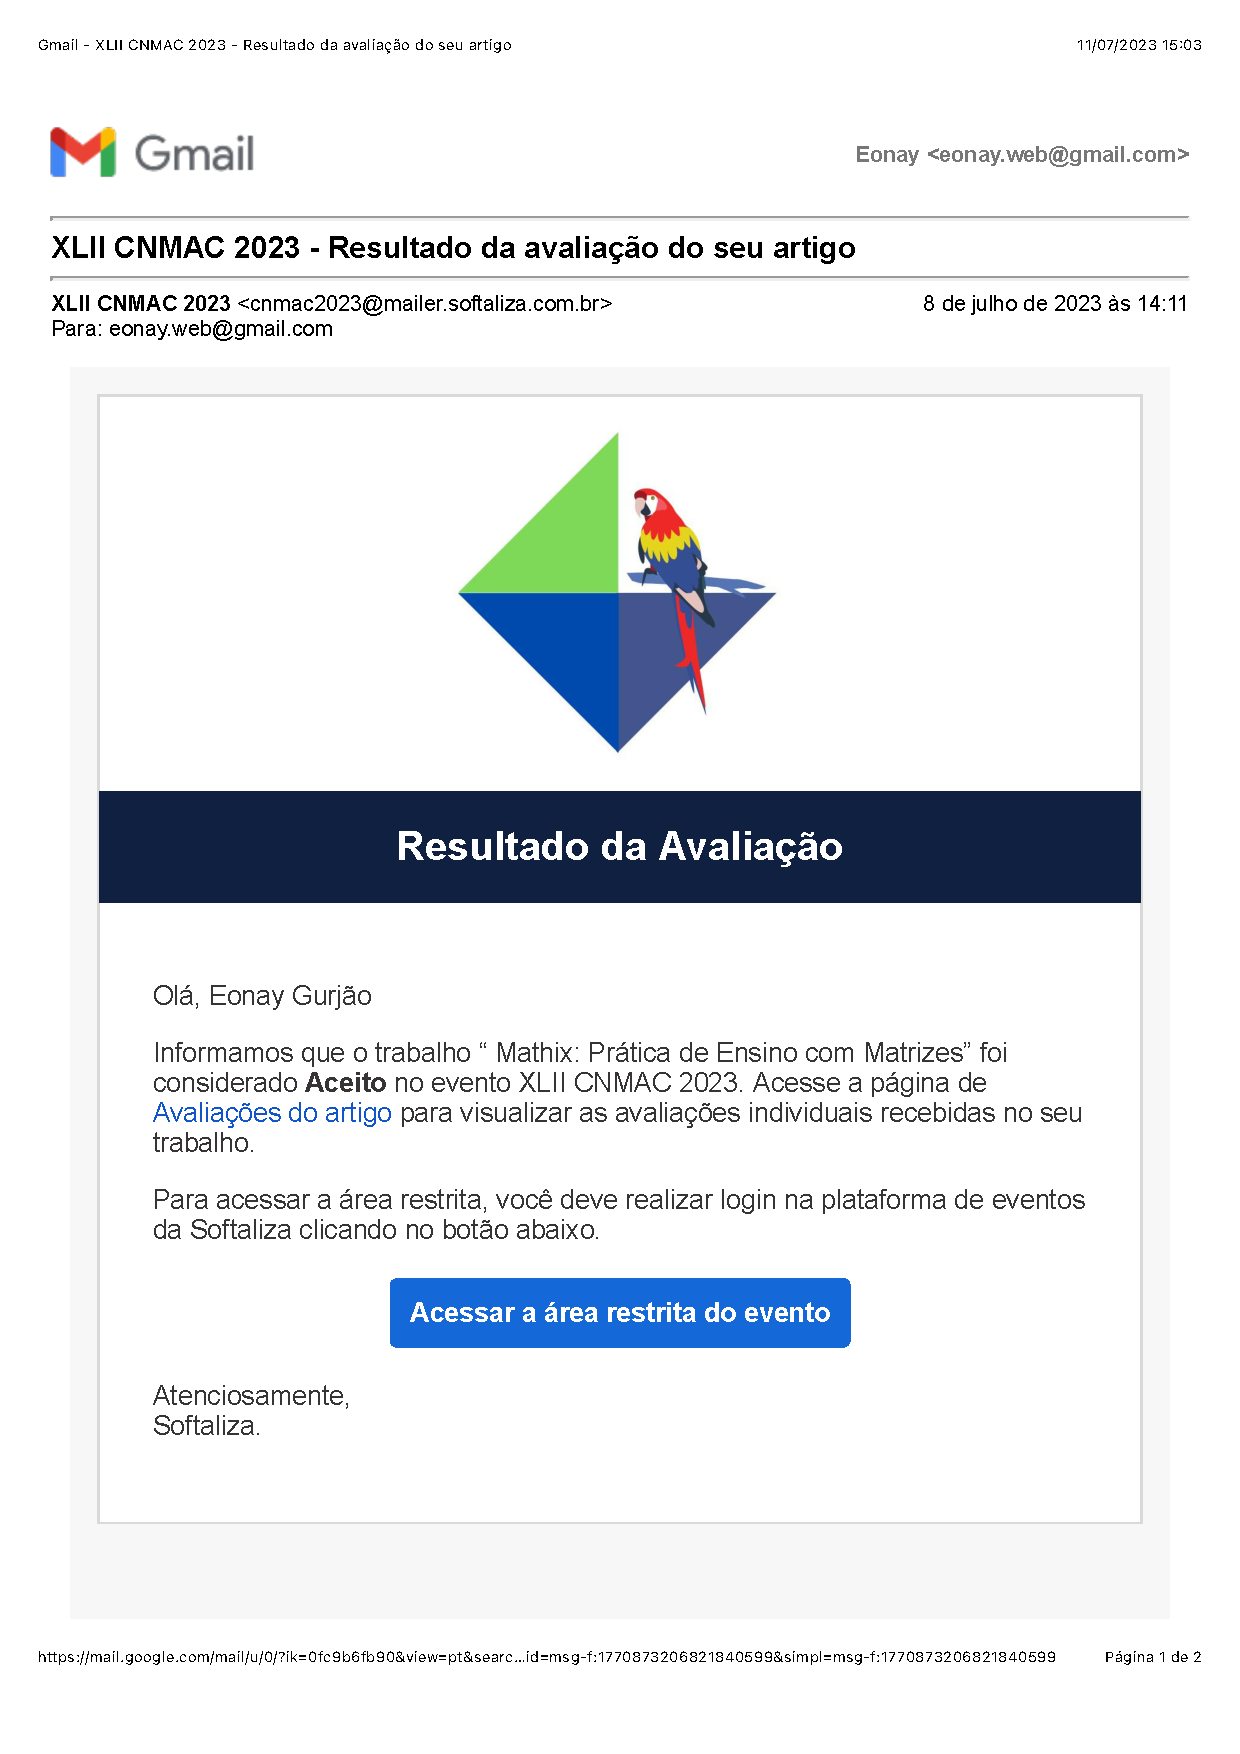
\includepdf[pages=-]{PosTextuais/submissao1.pdf}


% Anexo 04
\chapter{Submissão SENACEM 2024}
\begin{center}
    Documento recebido via Email para com a submissao do artigo para avaliação.    
\end{center}
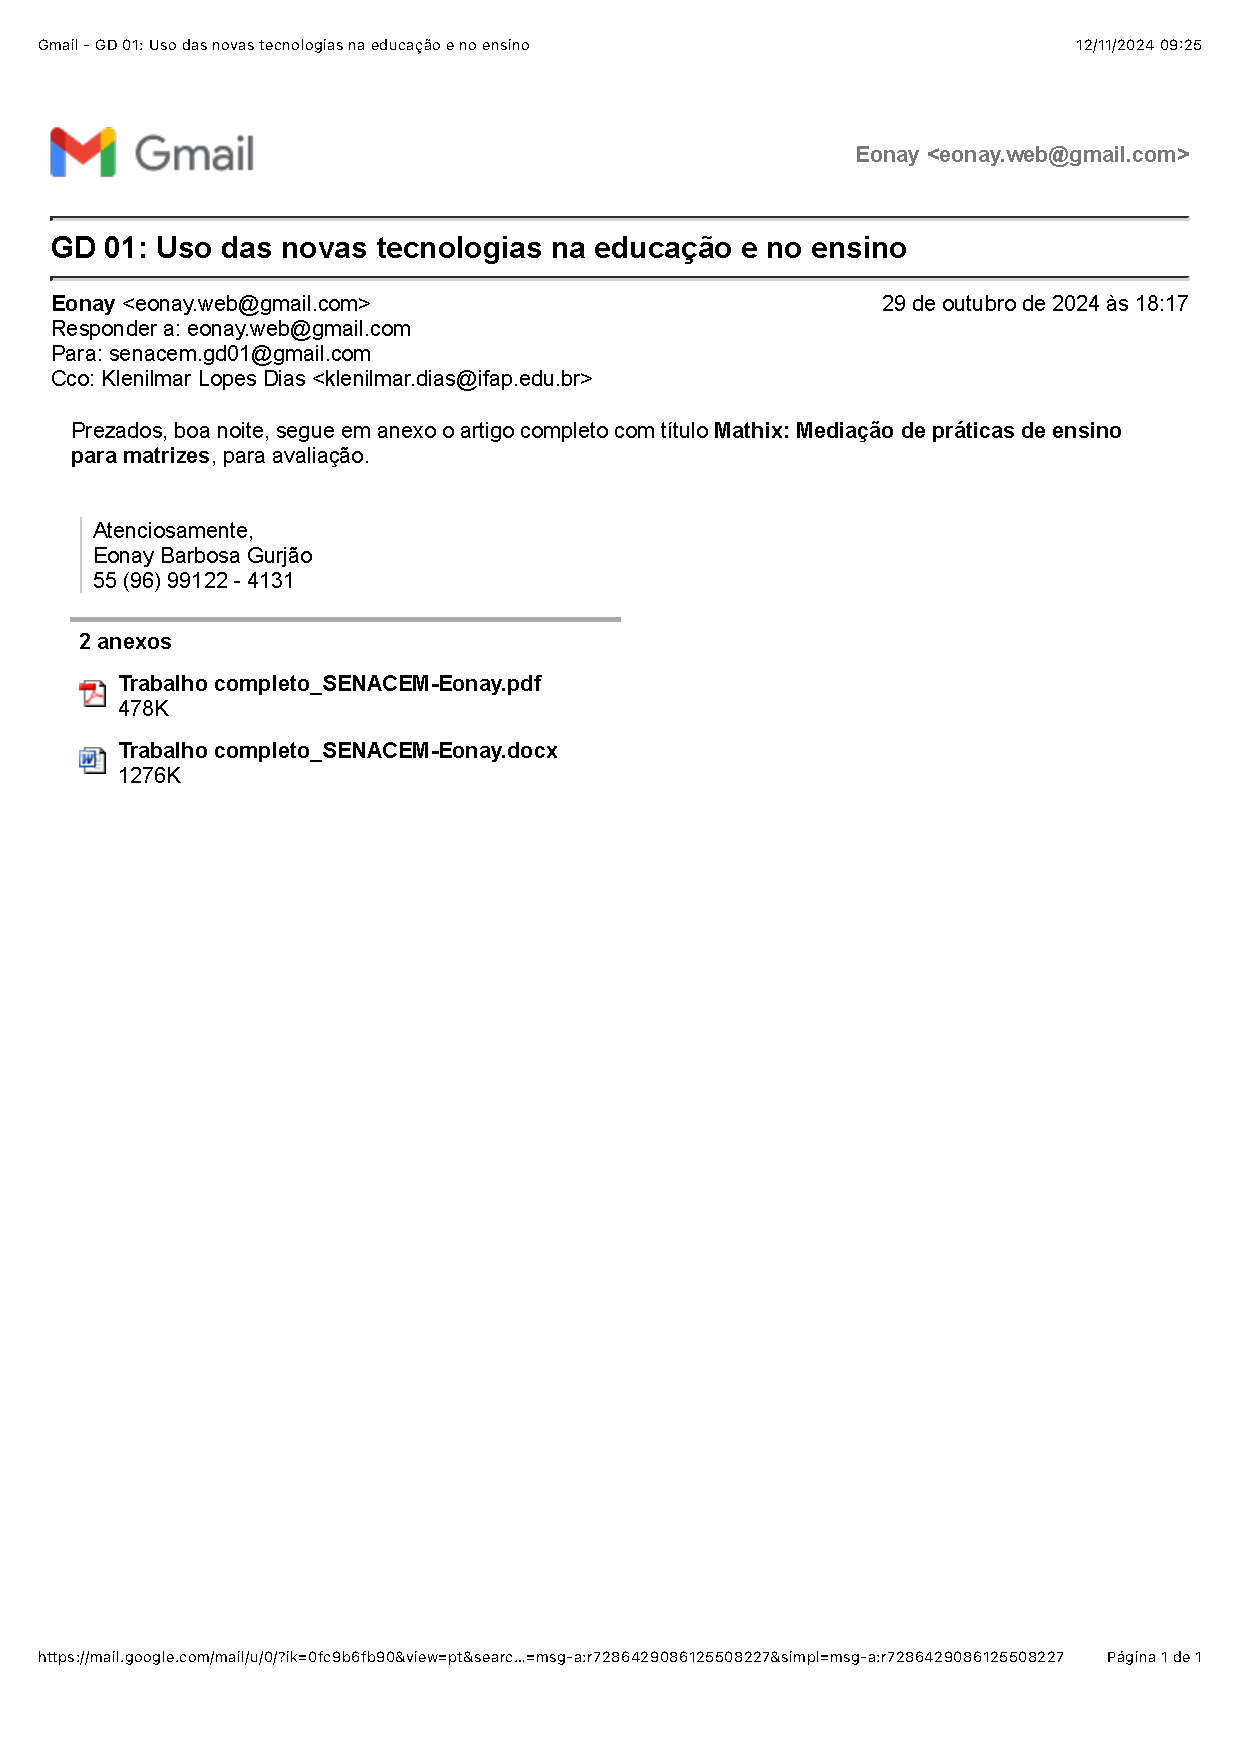
\includepdf[pages=-]{PosTextuais/submissao2.pdf}


% Anexo 05
\chapter{Relatório de Acesso aos Questionários }
\begin{center}
    Relatório de acesso aos questionário de avaliação emitidos via plataforma Survio.
\end{center}

\newpage
\begin{center}
    Relatório de acesso a avaliação do Produto Educacional.
    \newline
    \newline
    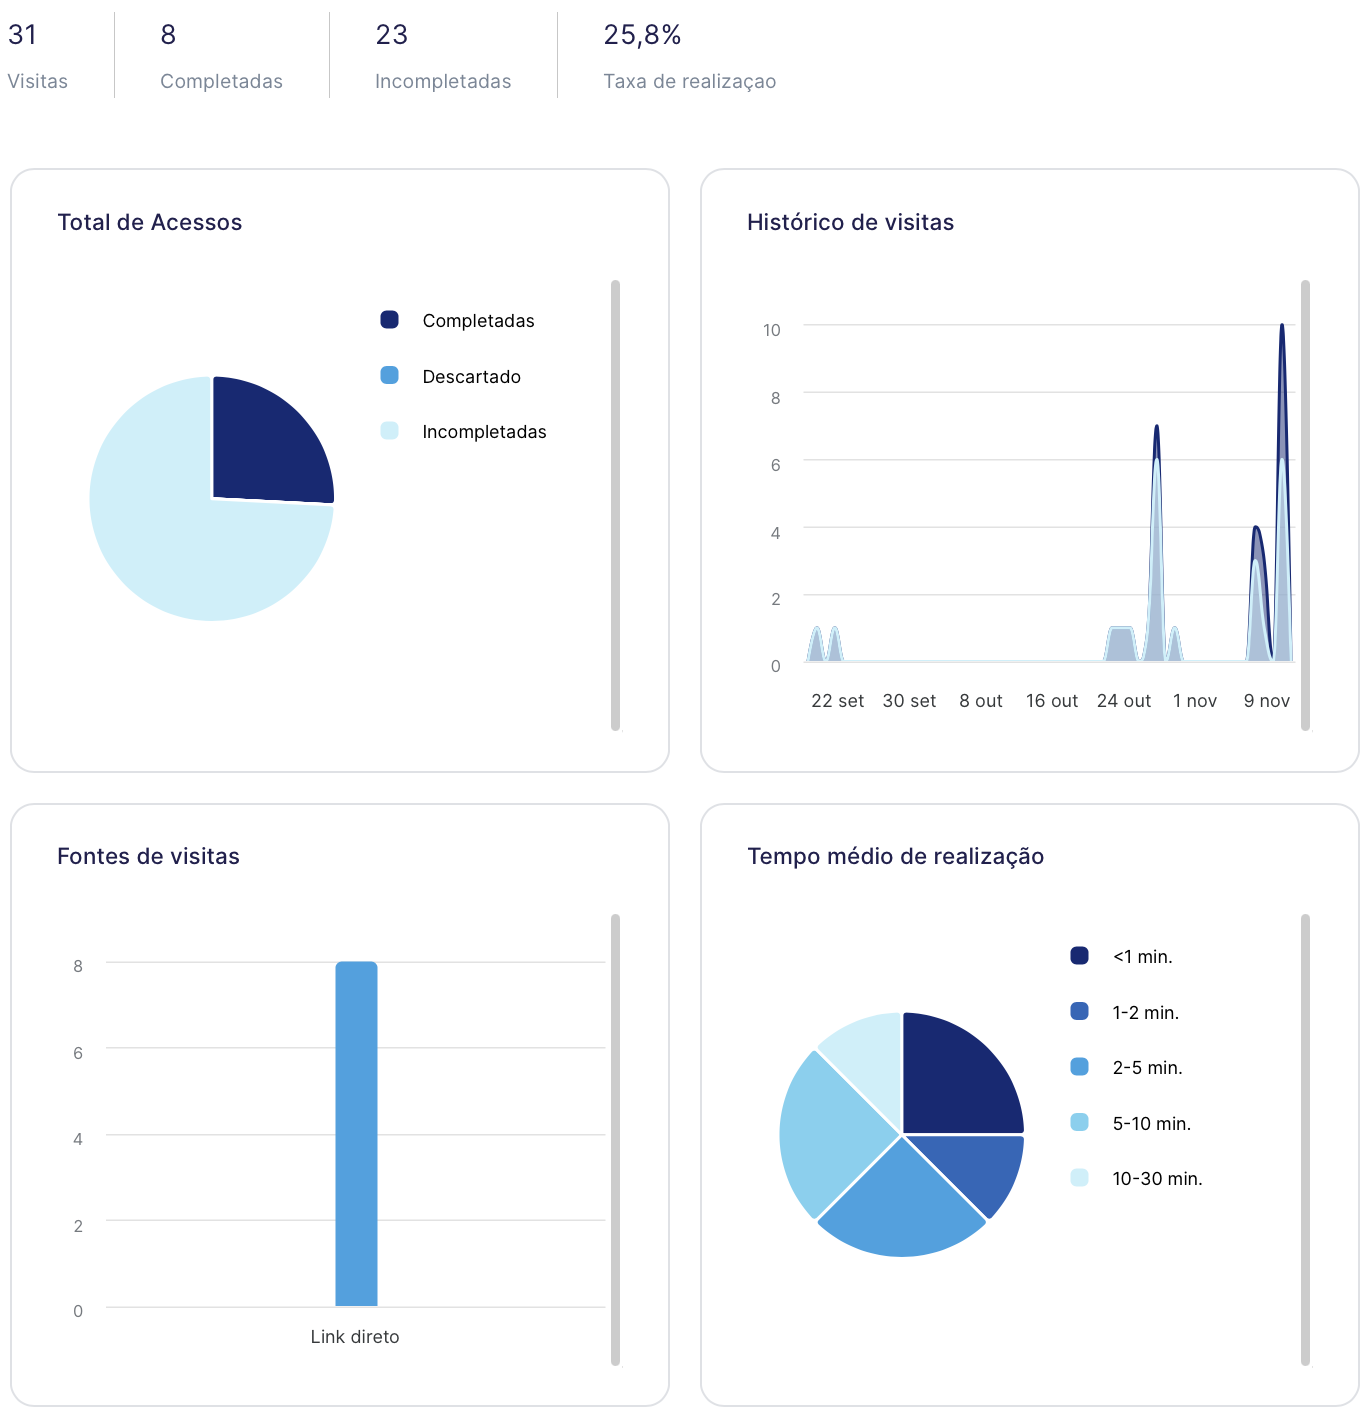
\includegraphics[width=\textwidth]{pos-textuais/anexo_pe.png}
\end{center}

\newpage
\begin{center}
    Relatório de acesso a avaliação de Interface de Usuário (UI) do Produto Educacional.
    \newline
    \newline
    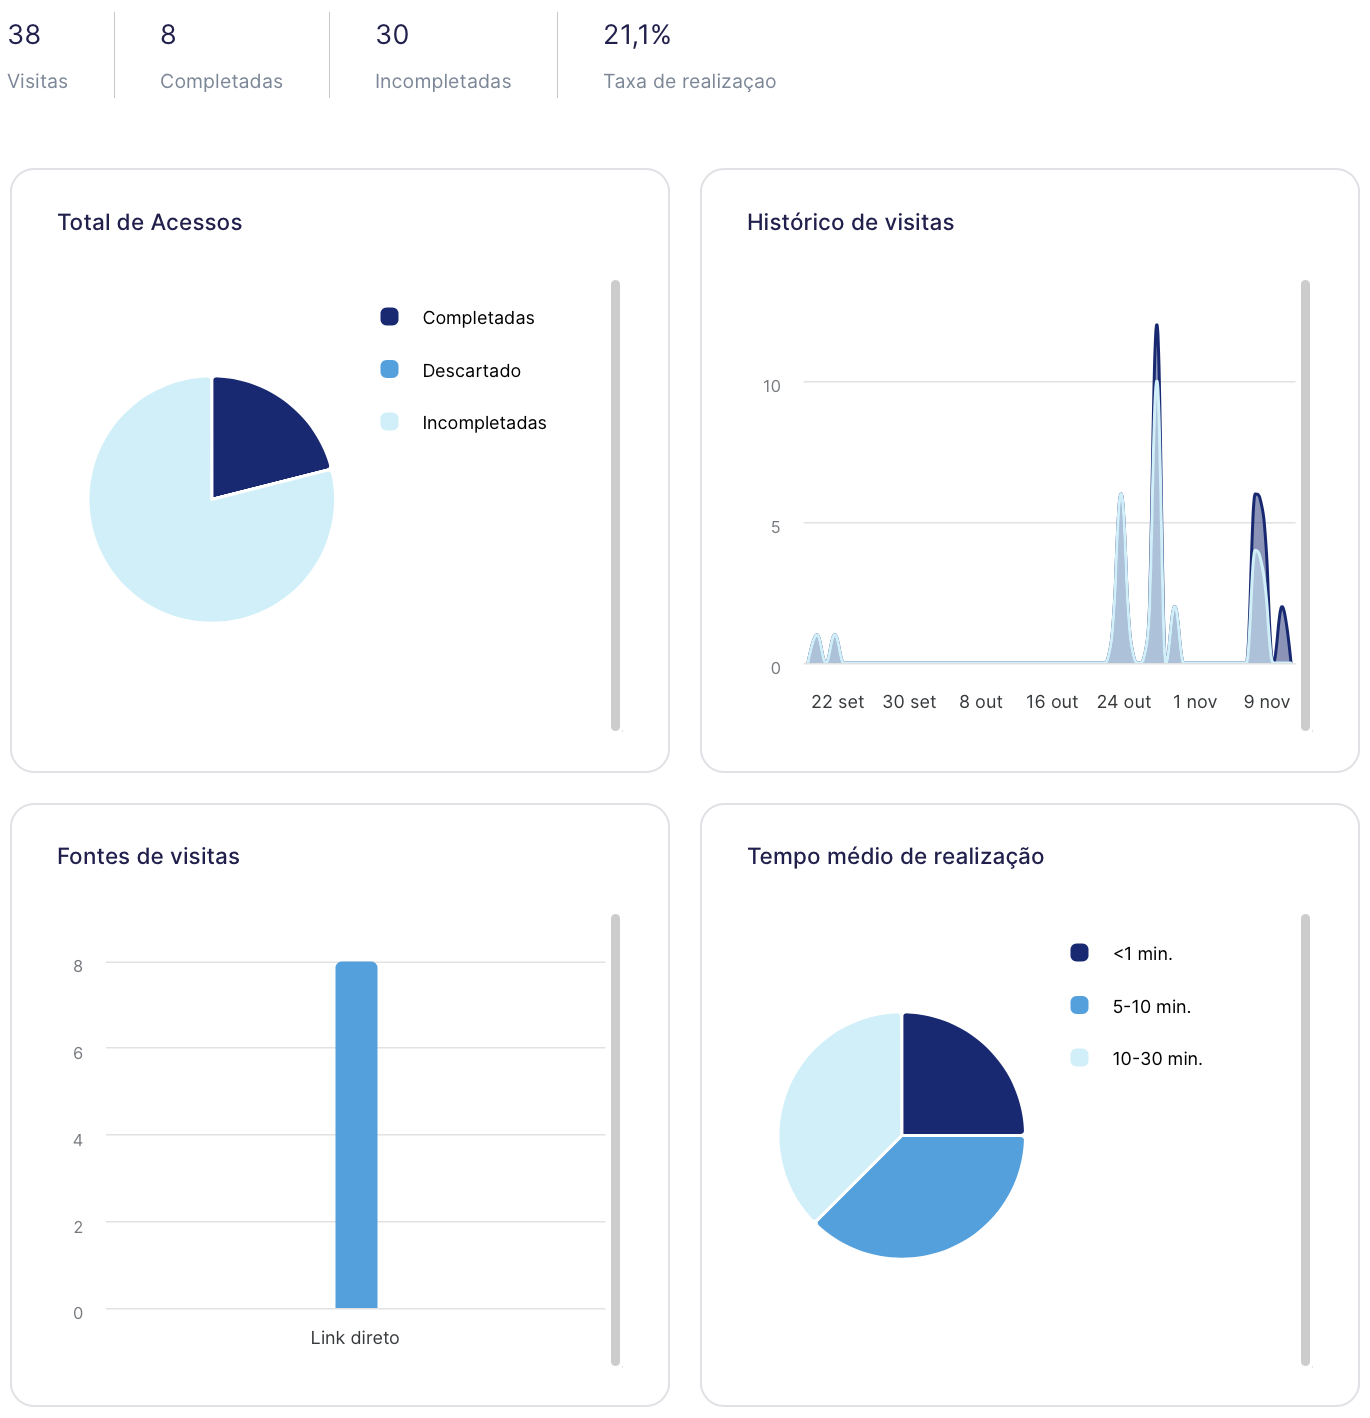
\includegraphics[width=\textwidth]{pos-textuais/anexo_ui.png}
\end{center}


\newpage
\begin{center}
    Relatório de acesso a avaliação de Experiência de Usuário (UX) do Produto Educacional.
    \newline
    \newline
    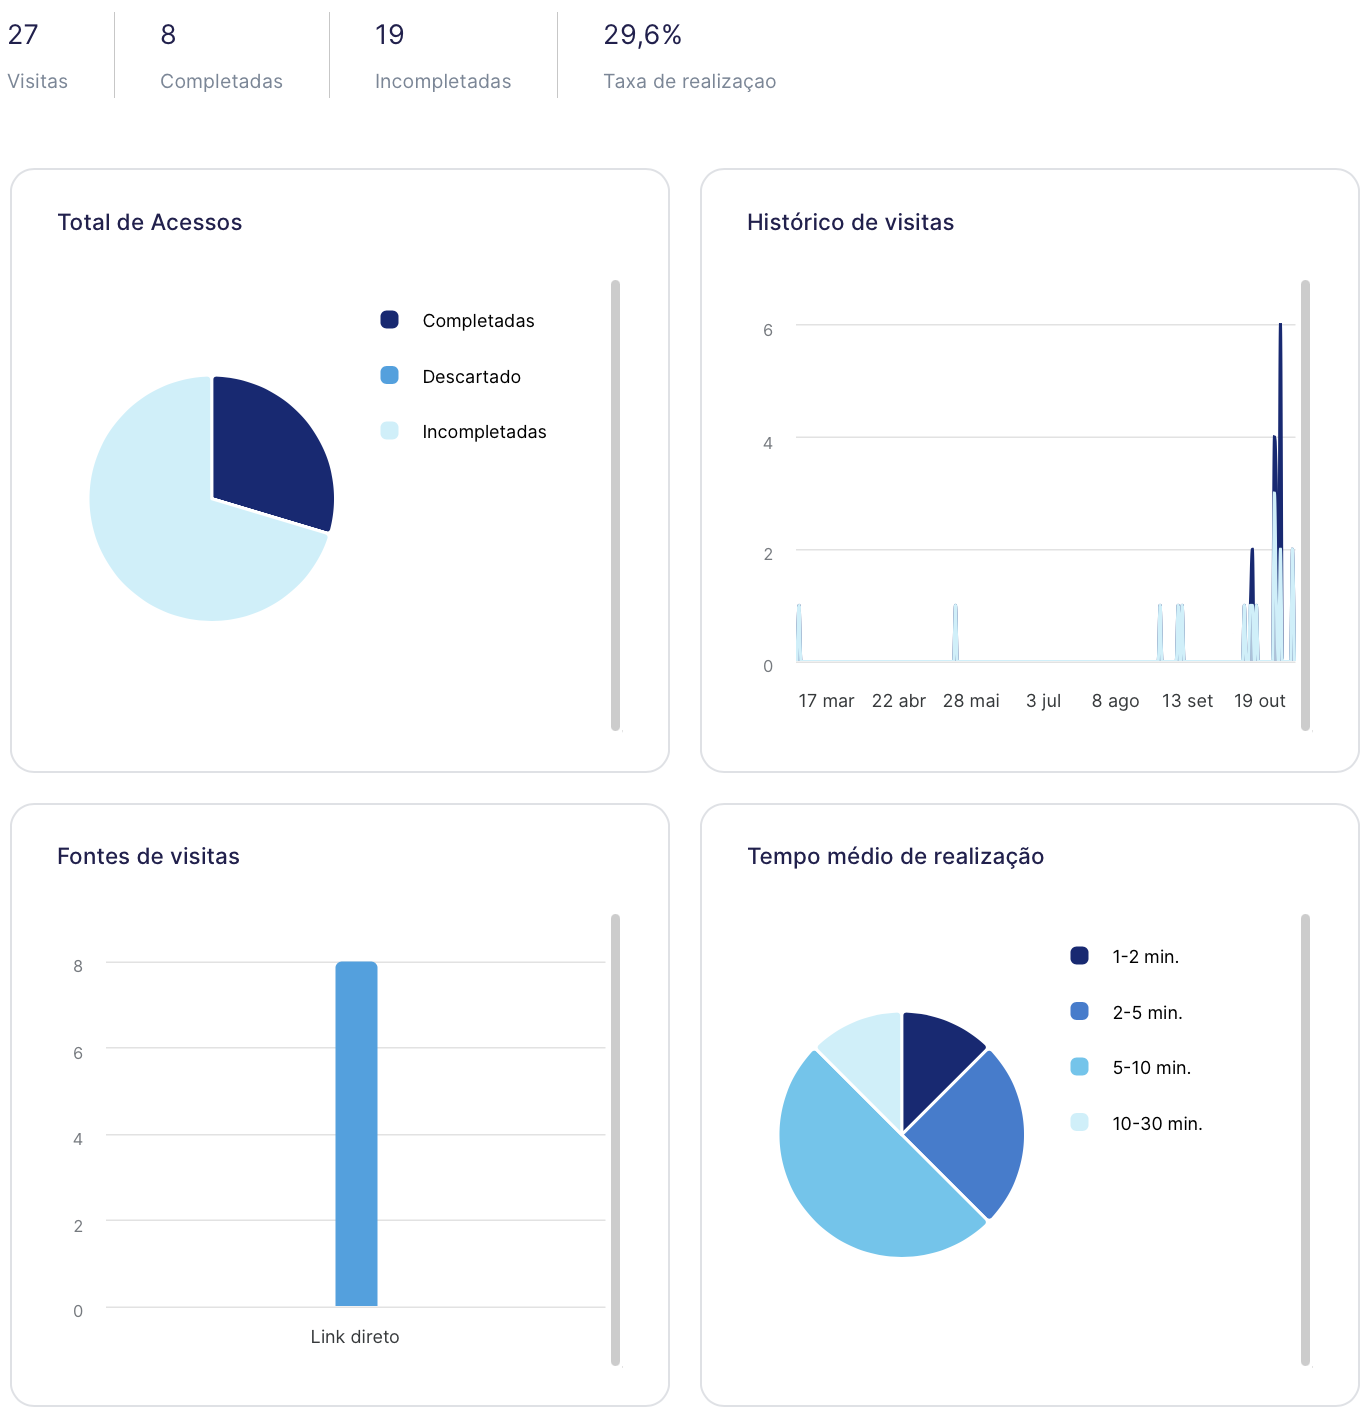
\includegraphics[width=\textwidth]{pos-textuais/anexo_ux.png}
\end{center}

\end{anexosenv}
